\documentclass{article}

\usepackage[utf8]{inputenc}

% Bibliography: Using natbib with BibTeX
\usepackage[english]{babel}
\usepackage[numbers]{natbib}                % Needed for the bibliography .bib file  
\bibliographystyle{plain}                   % BibTeX. Defaults: plain, unsrt, alpha, abbrv

\usepackage{tikz, pgfplots} % For drawing with tikz
\pgfplotsset{compat=1.18}       % Spesifies version

\usepackage{graphicx}       % Required for including RGB image files

% Bibliography: Using biblatex with biber
% \usepackage[backend=biber]{biblatex}      % Needed for the bibliography
% \addbibresource{references.bib}

\usepackage{url}            % Needed for URL links

%\usepackage{hyperref}      % Makes a reference into a hyperlink

\usepackage{multicol}       % For the multicolumn chapter
\usepackage{microtype}      % For the multicol chapter

\usepackage{amsthm}         % For theorems          (Settings in a file)

\usepackage{mdframed}       % For boxing equations and  theorems  (Settings in a file)

\usepackage{listings}       % Code formatting       (Settings in a file)
\usepackage{xcolor}         % Code formatting

\title{Graphics}
\author{Turkka Mella}
\date{March 2024}

\begin{document}
% Settings 
\input{Settings files/Settings - tikz}           % Needs to be first
% Note that these definitions are totally arbitrary, meaning that you could 
% define anything like this. For example you could have:
%   \theoremstyle{myAss}
%   \newtheorem{myAss}[theorem]{myAss}
% and you could use this with the syntax
%   \begin{myAss}
%   Let \( f: A \to B \) be a function from set \( A \) to set \( B \). If \( f \) is bijective, then there exists an inverse function \( f^{-1}: B \to A \).
%   \end{myAss}

% This defines 
%   - "theorem" to be the keyword in commands like: \begin{theorem} ... \end{theorem}
%   - "Theorem" to be the text that appears in the PDF with the numbering
%   - "section" to be the father category of theorem, so that children of theorem will be in the same 
%               numbering, meaning that if Lemma would be defined with syntax \newtheorem{lemma}{Lemma}[section]
%               it would have its own numbering, since now theorem is not its father but brother, hence they 
%               have now separate numberings.  
\newtheorem{theorem}{Theorem}[section]
\newtheorem{lemma}[theorem]{Lemma}
\newtheorem{corollary}[theorem]{Corollary}
\newtheorem{proposition}[theorem]{Proposition}

% The \theoremstyle{definition} command was used before defining the definition environment to 
% ensure that definitions are displayed differently (in upright text) than theorems, lemmas, 
% and corollaries (which are typically in italic text). The lemma did not need a \theoremstyle 
% command before it because lemmas, being similar to theorems in nature, use the default plain style, 
% which is already applied.
\theoremstyle{definition}
\newtheorem{definition}[theorem]{Definition}

\theoremstyle{remark}
\newtheorem{remark}[theorem]{Remark}

\theoremstyle{plain}
\newtheorem{plain}[theorem]{Plain}

% You can only use definition, remark, plain with this syntax since they are default. 
\mdfdefinestyle{equationframe}{
    linecolor=white,
    linewidth=1pt,
    leftmargin=10pt,
    rightmargin=10pt,
    backgroundcolor=gray!10,
    roundcorner=5pt
}
% Global settings for listings
\lstset{
    basicstyle=\ttfamily,
    commentstyle=\color{green},
    keywordstyle=\color{blue},
    stringstyle=\color{red},
    showstringspaces=false,
    identifierstyle=\color{black}
    % Removed procnamekeys
}

% Language-specific settings
\lstdefinestyle{cpp}{
    language=C++,
    breaklines=true,
    frame=single,
    numbers=left,
    numberstyle=\small,
    numbersep=8pt,
    showstringspaces=false,
    tabsize=2,
    morekeywords={auto} % Add additional C++ keywords here
}

\lstdefinestyle{python}{
    language=Python,
    breaklines=true,
    frame=single,
    numbers=left,
    numberstyle=\small,
    numbersep=8pt,
    showstringspaces=false,
    tabsize=2,
    morekeywords={def,class} % This is how you add extra keywords for Python
}


\maketitle
\tableofcontents                % Makes the table of contents

\section*{Abstract}
\addcontentsline{toc}{section}{Abstract}

This document provides an in-depth discussion on various LaTeX features. The abstract summarizes the contents of the document, giving readers an overview of what to expect. We explore the use of images, mathematical proofs, theorems, and multicolumn layouts. The aim is to demonstrate the versatility and power of LaTeX for typesetting complex documents.
    % Not numbered chapter
\section{Exploring Cubes with TikZ}

Cubes are one of the most fundamental shapes in both geometry and everyday life. Characterized by their six square faces, eight vertices, and twelve edges, cubes are a prime example of a three-dimensional square. They can be found in various contexts, from architecture and design to natural formations. In mathematics, cubes are studied not only for their geometric properties but also for their applications in algebra, where the cube of a number is its third power.

\begin{figure}[ht]
\centering % Centers the figure
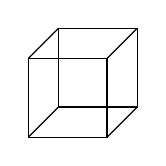
\begin{tikzpicture}
    % Bottom face
    \draw (0,0,0) -- (1,0,0) -- (1,1,0) -- (0,1,0) -- cycle;
    % Top face
    \draw (0,0,1) -- (1,0,1) -- (1,1,1) -- (0,1,1) -- cycle;
    % Side edges
    \draw (0,0,0) -- (0,0,1);
    \draw (1,0,0) -- (1,0,1);
    \draw (1,1,0) -- (1,1,1);
    \draw (0,1,0) -- (0,1,1);
\end{tikzpicture}
\caption{A simple 3D cube drawn with TikZ.} % Adds your caption here
\label{fig:3dcube} % Labels the figure for cross-referencing
\end{figure}

The cube illustrated above is created using TikZ, a powerful tool for generating vector graphics directly in LaTeX documents. Through simple commands, TikZ allows for precise control over the drawing, enabling the creation of both simple diagrams like this cube and more complex figures. The cube's representation here, while simple, serves as a foundational example for more intricate geometric constructions and visualizations in LaTeX. Learning to draw with TikZ not only enhances your documents visually but also provides a deeper understanding of the geometric concepts being presented.
       % Draw image example
\section{An Essay on Apples}

Apples are among the most popular and beloved fruits worldwide. Known scientifically as Malus domestica, apples have been cultivated by humans for thousands of years. Originating in Central Asia, these fruits have spread to every corner of the globe and have been embraced in various cultures, cuisines, and traditions.

Apples come in a wide variety of flavors, colors, and textures, ranging from sweet to tart and from crisp to soft. This diversity has allowed apples to be incredibly versatile in cooking and baking, featuring in dishes from simple snacks like raw apple slices to complex recipes like apple pies and tarts.

Beyond their culinary uses, apples have significant cultural and symbolic meanings. They can represent knowledge, as seen in the story of Adam and Eve, or temptation and desire. In many cultures, apples are a symbol of health and vitality, encapsulated in the saying, "An apple a day keeps the doctor away."

Nutritionally, apples are a rich source of fiber, vitamin C, and various antioxidants. These nutrients contribute to various health benefits, such as improving digestion, enhancing heart health, and potentially reducing the risk of chronic diseases.

The cultivation of apples is a significant industry in many countries, with China, the United States, and Poland being among the top producers. The process of growing apples, from planting and pruning to harvesting and storage, requires careful management to ensure the quality and yield of the fruit.

In conclusion, apples are not just a staple in diets around the world but also carry deep cultural and symbolic significances. Their widespread popularity is a testament to their versatility, nutritional value, and the joy they bring to people's lives.

\begin{table}[ht]
\centering
\begin{tabular}{l|l|l}
Type & Color & Taste \\
\hline
Granny Smith & Green & Tart \\
Gala & Red & Sweet \\
Honeycrisp & Red/Yellow & Crisp \\
\end{tabular}
\caption{Types of Apples and Their Characteristics}
\label{table:apples}
\end{table}       % Essey example
\section{A New Chapter on Equations}

This chapter introduces some fundamental equations in physics.

The first equation is Newton's second law, which states that the force applied to an object is equal to the mass of the object multiplied by its acceleration.

\begin{equation}
F = ma
\label{eq:NewtonII} % This makes it possible to reference to this equation
\end{equation}

This law is a cornerstone in classical mechanics.

Next, we consider the equation for gravitational force, which describes the attraction between two masses.

\begin{mdframed}    % This is now boxed equation
\begin{equation}
F = G \frac{m_1 m_2}{r^2}
\label{eq:gravity} % This makes it possible to reference this equation
\end{equation}
\end{mdframed}

Where $G$ is the gravitational constant, $m_1$ and $m_2$ are the masses of the two objects, and $r$ is the distance between their centers.

Lastly, we look at the equation for kinetic energy, which represents the energy that an object possesses due to its motion.

\begin{equation}
KE = \frac{1}{2} mv^2
\label{eq:kineticEnergy} % This makes it possible to reference to this equation
\end{equation}

Where $m$ is the mass of the object and $v$ is its velocity.

Inserting a new equation between these will automatically update the numbering without any additional adjustments needed.    % Equation example
\section{Referencing Examples}

One of the fundamental aspects of LaTeX is its ability to handle references dynamically. This feature is particularly useful when dealing with mathematical equations, figures, tables, and even sections of text, such as appendices. A prime example of this is Equation~\ref{eq:gravity}, which introduces the concept of gravitational force. Similarly, we can reference sections of our document, such as the appendix on Nikola Tesla, which can be found in Appendix~\ref{app:Tesla}. The ability to reference dynamically ensures that our text always points to the correct equation or section, regardless of any modifications that might occur in the document structure.


   % Reference example   
\input{Chapter files/Chapter - Citations}   % Citation example    
\section{Understanding Footnotes}

Footnotes are an essential part of academic and research writing, offering a convenient way to provide additional information, clarifications, or references without cluttering the main text. They allow authors to elaborate on specific points without interrupting the flow of their arguments or narrative\footnote{Footnotes appear at the bottom of the page on which they are referenced, making it easy for readers to find supplementary information without losing their place in the text.}.

The use of footnotes is not limited to academic writing; it is also prevalent in books, reports, and other documents where detailed explanations or citations are necessary. They contribute significantly to the depth and richness of a document, enabling writers to substantiate their claims and readers to explore topics further.

In LaTeX, the \textbackslash{}footnote command simplifies the process of adding footnotes, automatically handling numbering and placement, thus maintaining the document's integrity and readability.
    % Footnote example
\section{RGB image example}

In this section, we include an external graphic into our document. This can be an image file such as a JPEG, PNG, or PDF. The figure below demonstrates how an image is included using LaTeX.

\begin{figure}[htbp]
\centering
\includegraphics[width=0.8\textwidth]{66.png} % Updated to the correct image file name

\caption{The included image.} % Caption for the image
\label{fig:external-graphic} % Label used for referencing the figure in-text
\end{figure}

As shown in Figure~\ref{fig:external-graphic}, you can reference figures easily in your text.
    % External image example 
\input{Chapter files/Chapter - Multi column}% Multi column example    
\section{Mathematical Proofs and Theorems}

Mathematical proofs and theorems are the core components of any mathematical text. They provide the logical foundation upon which mathematical theory is built. LaTeX, with the help of packages like `amsthm`, provides an excellent way to typeset these structures.

\subsection{Sample Theorem}
% To have this boxed  
\begin{mdframed}
\begin{theorem}
    If \( f: A \to B \) is bijective, then there exists an inverse function \( f^{-1}: B \to A \).
\end{theorem}
\end{mdframed}

\begin{theorem}
Let \( f: A \to B \) be a function from set \( A \) to set \( B \). If \( f \) is bijective, then there exists an inverse function \( f^{-1}: B \to A \).
\end{theorem}

\begin{proof}
Since \( f \) is bijective, for each \( b \in B \), there exists a unique \( a \in A \) such that \( f(a) = b \). We define \( f^{-1}(b) = a \). To show that \( f^{-1} \) is the inverse of \( f \), we must demonstrate that \( f(f^{-1}(b)) = b \) for all \( b \in B \) and \( f^{-1}(f(a)) = a \) for all \( a \in A \).

First, we show that \( f(f^{-1}(b)) = b \) for all \( b \in B \). Since \( f^{-1}(b) = a \), it follows that \( f(f^{-1}(b)) = f(a) = b \).

Next, we show that \( f^{-1}(f(a)) = a \) for all \( a \in A \). Since \( f(a) = b \), and \( f^{-1}(b) = a \), it follows that \( f^{-1}(f(a)) = f^{-1}(b) = a \).

Therefore, \( f^{-1} \) is the inverse function of \( f \).
\end{proof}

\subsection{Sample Lemma}
\begin{lemma}
For every non-empty set \( S \), if \( f: S \to S \) is injective, then \( f \) is surjective.
\end{lemma}

\begin{proof}
(Sketch) Since \( S \) is non-empty and \( f \) is injective, every element of \( S \) maps to a distinct element of \( S \). Given the finiteness of \( S \), this implies that \( f \) must cover all elements of \( S \), hence it is surjective.
\end{proof}


\subsection{Sample Corollary}
\begin{corollary}
If \( f: A \to B \) and \( g: B \to C \) are bijective functions, then the composition \( g \circ f: A \to C \) is also bijective.
\end{corollary}

\begin{proof}
Omitted for brevity.
\end{proof}

\subsection{Sample Definition}
\begin{definition}
A function \( f: A \to B \) is said to be \emph{injective} if for every \( a_1, a_2 \in A \), \( f(a_1) = f(a_2) \) implies that \( a_1 = a_2 \).
\end{definition}

\subsection{Sample Remark}
\begin{remark}
This is a remark that provides additional information or context about the material presented above.
\end{remark}
     % Theorems example
\section{Programming Examples}

This chapter includes examples of code in both C++ and Python. These examples are designed to demonstrate basic syntax and concepts in each language.

\subsection{C++ Example}
The following C++ example shows a simple "Hello, World!" program:

\begin{lstlisting}[style=cpp]
#include <iostream>

int main() {
    std::cout << "Hello, World!" << std::endl;
    return 0;
}
\end{lstlisting}

\subsection{Python Example}
The following Python example demonstrates a simple script that prints "Hello, World!" to the console:

\begin{lstlisting}[style=python]
print("Hello, World!")
\end{lstlisting}

Both examples illustrate the basic structure of a program in their respective languages.
        % Code example

Relativity \cite{einstein2013principle} and such as that.

\appendix
\section{Newton}
\label{app:Newton}

Sir Isaac Newton was a key figure in the scientific revolution, known for his laws of motion and universal gravitation. His work laid the foundation for classical mechanics and has influenced many areas of mathematics, physics, and astronomy. Newton's contributions extend beyond the well-known apple anecdote, profoundly shaping our understanding of the natural world.
 % THESE NEED TO BE input AND NOT include, because otherwise bibliography gives errors
\section{Nikola Tesla}
\label{app:Tesla}

Nikola Tesla was a pioneering inventor and engineer known for his groundbreaking work on alternating current (AC) electrical systems. He developed the AC motor and contributed to the establishment of AC as the standard for electric power transmission worldwide. Tesla's passion for discovery led to numerous innovations in the fields of electrical and radio engineering, leaving a lasting legacy.


\bibliography{references}
\addcontentsline{toc}{section}{References} % References to table of contents
% \nocite{*} This command shows all the source for citations even if they aren't used

\end{document}